\documentclass[15pt]{article}

% if you need to pass options to natbib, use, e.g.:
%     \PassOptionsToPackage{numbers, compress}{natbib}
% before loading neurips_2018

% ready for submission
% \usepackage{neurips_2018}

% to compile a preprint version, e.g., for submission to arXiv, add add the
% [preprint] option:
%     \usepackage[preprint]{neurips_2018}

% to compile a camera-ready version, add the [final] option, e.g.:
     \usepackage[final]{neurips_2018}
     

% to avoid loading the natbib package, add option nonatbib:
%     \usepackage[nonatbib]{neurips_2018}

\usepackage[utf8]{inputenc} % allow utf-8 input
\usepackage[T1]{fontenc}    % use 8-bit T1 fonts
\usepackage{hyperref}       % hyperlinks
\usepackage{url}            % simple URL typesetting
\usepackage{booktabs}       % professional-quality tables
\usepackage{amsfonts}       % blackboard math symbols
\usepackage{nicefrac}       % compact symbols for 1/2, etc.
\usepackage{microtype}      % microtypography
\usepackage[english]{babel}
\usepackage{hanging} % for hanging references
\usepackage{physics} % for bra ket notation
\usepackage{graphicx}
\usepackage{caption}
\usepackage{subcaption}
\usepackage{float}
\usepackage{wrapfig}
\usepackage{listings}
\graphicspath{ {./images/} }

\title{Project 3 Report}

% The \author macro works with any number of authors. There are two commands
% used to separate the names and addresses of multiple authors: \And and \AND.
%
% Using \And between authors leaves it to LaTeX to determine where to break the
% lines. Using \AND forces a line break at that point. So, if LaTeX puts 3 of 4
% authors names on the first line, and the last on the second line, try using
% \AND instead of \And before the third author name.

\author{%
  Yizhan Ao\\
  Email: josephao@umd.edu   \\
  UID: 116022064\\
  \And
  Yingqiao Gou\\
  Email: ygou@terpmail.umd.edu\\
  UID: 115979000\\
}

\begin{document}
 
\maketitle

\begin{abstract}
We used 4 late days
\end{abstract}

\section{Concept}
The aim of this project is to segment deformable object from a given video sequence. This document just provides an overview of what you need to do. For a full breakdown of how each step in the pipeline works, see the course notes for this project.

\section{Setting up local windows}
Finding and saving the window's midpoints was all that was required to initialize the local windows. These mid-points were just points uniformly dispersed over the first mask's shape. InitLocalWindows.m has previously done this for us. We didn't alter anything except the problem that was in the code at the time.
\\
\begin{subfigure}{.5\textwidth}
  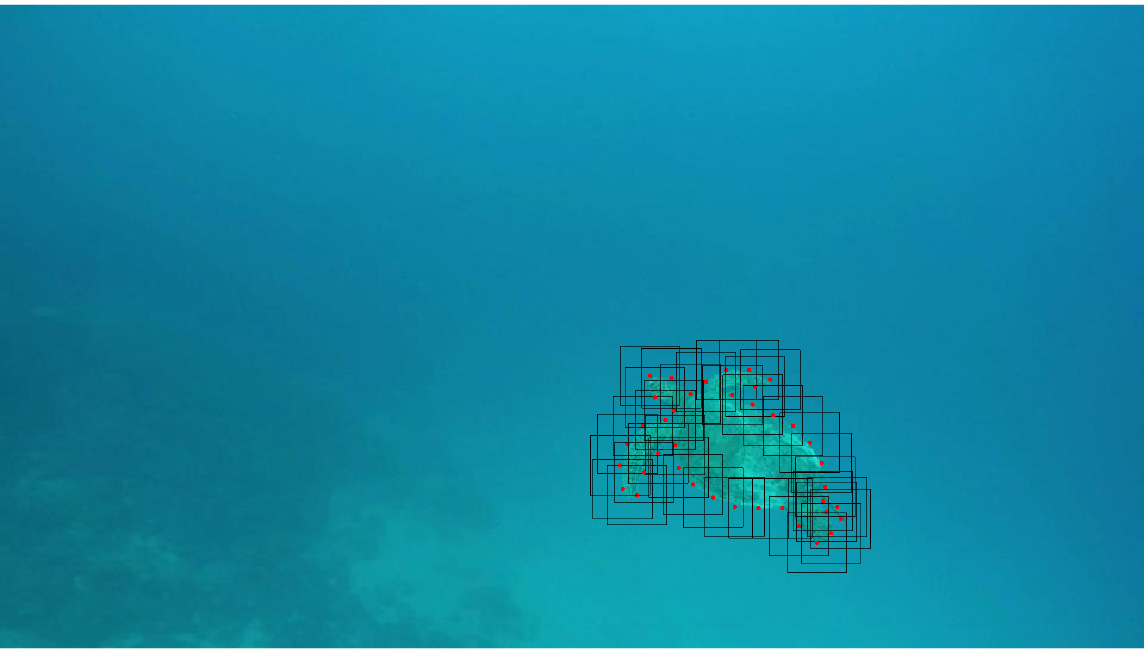
\includegraphics[width=140mm]{images/initialize the local windows.png}
  \caption{Color Confidence example }
  \label{fig:sub1}
\end{subfigure}%


\section{Initializes color models}
We used rgb2lab to convert the original frame from RGB to LAB colorspace in order to initialize the color models. Then, using bwdist, to calculate the distance matrix of the mask outline in each window. This provides me the distance to the original mask's edge, which allows us to eliminate points that are too near to the edge from GMM training since color changes dramatically at this edge and may not be representational of either the foreground or background.
\begin{equation}
p_{c}(x)=p_{c}(x \mid \mathcal{F}) /\left(p_{c}(x \mid \mathcal{F})+p_{c}(x \mid \mathcal{B})\right)
\end{equation}
The color model is started by estimating a Gaussian Mixture Model for each window's foreground pixels, and then computing a GMM for the background pixels (where the mask is produced by the user's roipoly result). Because there is little change in the colors of the foreground and background in the instance of the turtle, we utilized GMM of size 1; the number k varied for the other sets of photos.
\section{Initializes color confidences}
The color confidence is derived using the Rotobrush paper's algorithm and is dependent on the color model. Every window's color confidences are saved. [0,1] is a nice method to represent how effectively the foreground and background are separated.


\begin{equation}
f_{c}=1-\frac{\int_{W_{k}}\left|L^{t}(x)-p_{c}(x)\right| \cdot \omega_{c}(x) d x}{\int_{W_{k}} \omega_{c}(x) d x}
\end{equation}
\begin{subfigure}{.5\textwidth}
  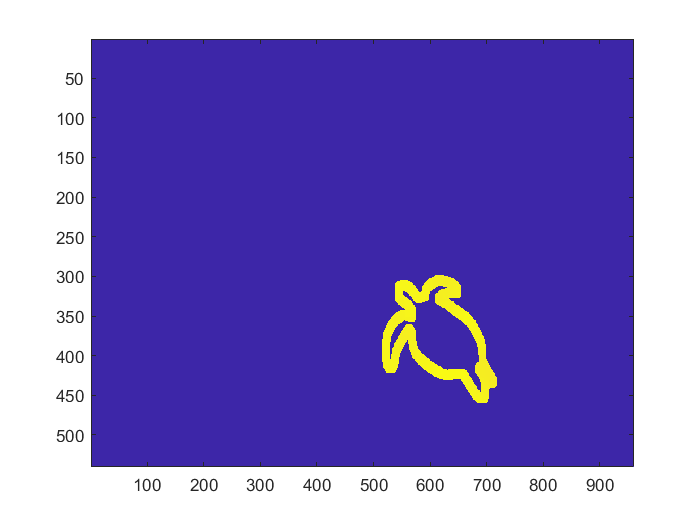
\includegraphics[height=100mm\linewidth,center]{images/the color confidences.png}
  \caption{Color Confidence example }
  \label{fig:sub1}
\end{subfigure}%
\section{Shapes Models}
\begin{equation}
f_{s}(x)=1-\exp \left(-d^{2}(x) / \sigma_{s}^{2}\right)
\end{equation}
To update foreground GMM, we sampled all pixels in the warped window whose foreground confidence estimated from the update shape model is greater than a high threshold 0.75, according to the paper. Because ShapeConfidence simply keeps track of the confident score in relation to the windows, When the window is deformed, it is updated. To train a GMM model for the current frame, we only need to cycle through every pixel in every previous warped window that has a shape confidence score greater than 0.75 to feed into the GMM model.

\subsection{How to Update Shape Model}
\begin{equation}
\sigma_{s}=\left\{\begin{array}{cl}
\sigma_{\min }+a\left(f_{c}-f_{\text {cutoff }}\right)^{r} & f_{\text {cutoff }}<f_{c} \leq 1 \\
\sigma_{\min } & 0 \leq f_{c} \leq f_{\text {cutoff }}
\end{array}\right.
\end{equation}
The paper discusses the two sigma cases in Formula 4. I assume that has been addressed in the function because the shape model is dependent on the initShapeConfidences() Then we do simply compare the total number of foreground pixels in the prior and current GMMs after the update.
\begin{lstlisting}
for (every shape confidences):
    use color confidences and sigma to do some calculations...
    ShapeConfidences.Confidences{i} = new_f_s;
    % This is from the Piazza that is very helpful to us!
\end{lstlisting}

\subsection{How to find the foreground probability of each window}
\begin{equation}
p_{\mathcal{F}}^{k}(x)=f_{s}(x) L^{t+1}(x)+\left(1-f_{s}(x)\right) p_{c}(x)
\end{equation}
Every window must be iterated through to determine the foreground probability of each pixel. The $pkF(x)$ cellular array would be a 1xWindows count cellular array that stores the pixels' WidthxWidth foreground probability. When we utilize the warped mask here, we must first remove the appropriate patch from the current window.
\begin{lstlisting}
current_mask_window = warpedMask(current_window_xRange, current_window_yRange);
\end{lstlisting}


\section{Updating Window Locations}
We utilized detectSURFFeatures, which is rotational invariant, to estimate the vast quantities of motion in the object. We tried deleting the backdrop (setting pixels to NaN) to compel matching to focus on the foreground, however this frequently resulted in the algorithm failing to discover enough matching sites. Even with an iterative matching threshold, we were unable to resolve this issue. Even if there were matches early on, the algorithm would eventually fail. This, we believe, is the major source of the algorithm's failure in rotating frame sets. Some of the matches are fine, while some are terrible, resulting in a bad transformation, as illustrated below. We think one of the things we shouldn't spend too much time on is that twerking the parameters(including the size of the window and numbers of the windows). I think we have tried too hard to find the best result of the window positioning. 

\section{Calculates local window movement based on optical flow between frames}
This step is to estimate the local boundry and deform the picture. The transformation was insufficient to track modest amounts of motion. To account for these little variations, we employed optical flow. We determined the average optical flow in the X and Y directions for the foreground pixels in each window and added it to the points in that window.
\section{Results}

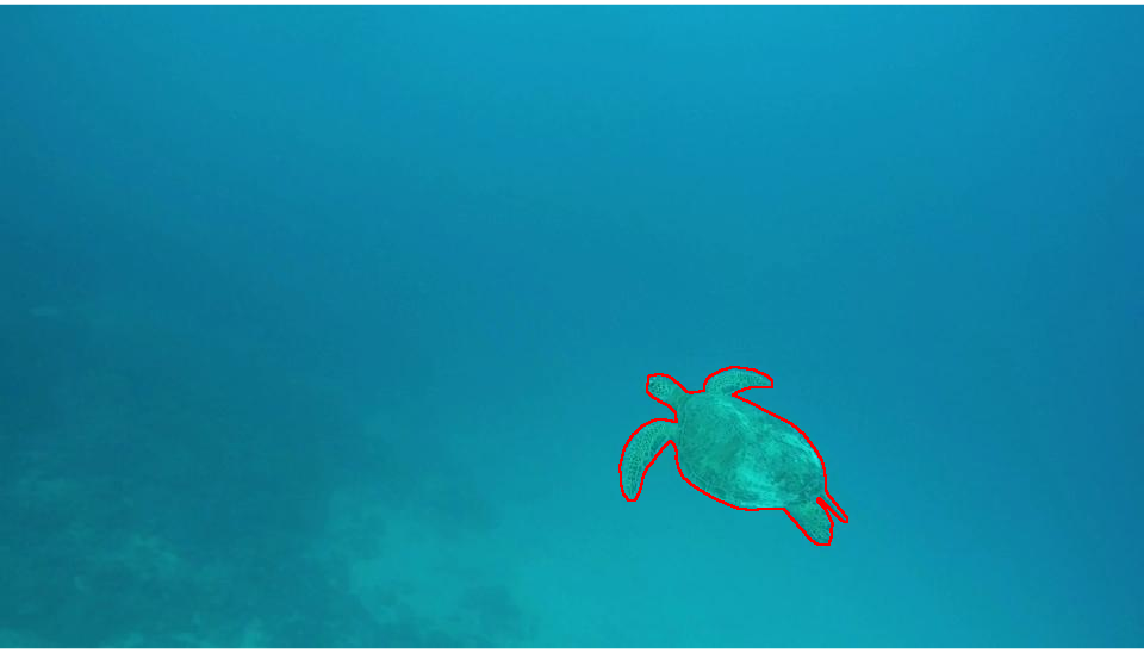
\includegraphics[width= 70mm]{images/initialize the mask.png}
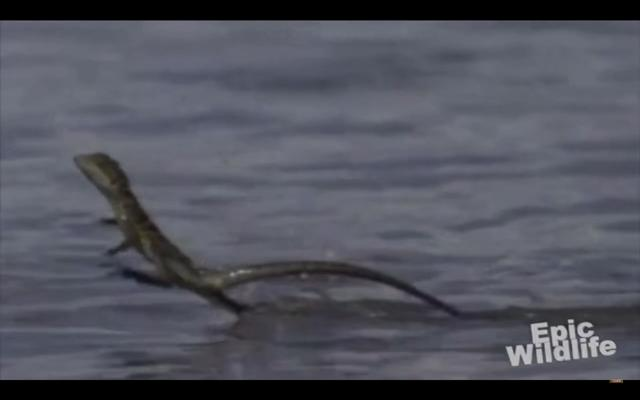
\includegraphics[width= 73mm]{images/2.jpg}
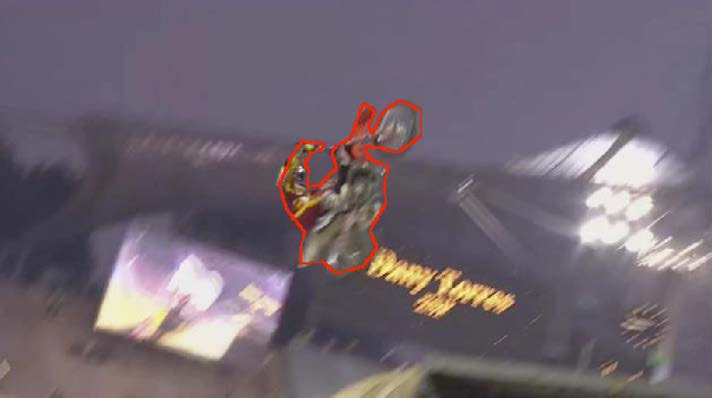
\includegraphics[width= 70mm]{images/3.jpg}
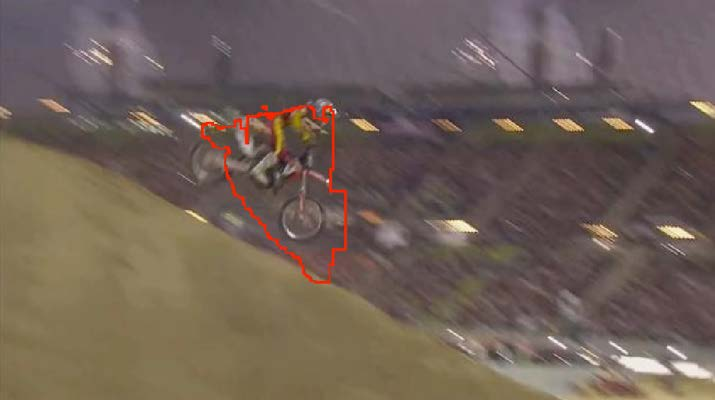
\includegraphics[width= 73mm]{images/4.jpg}
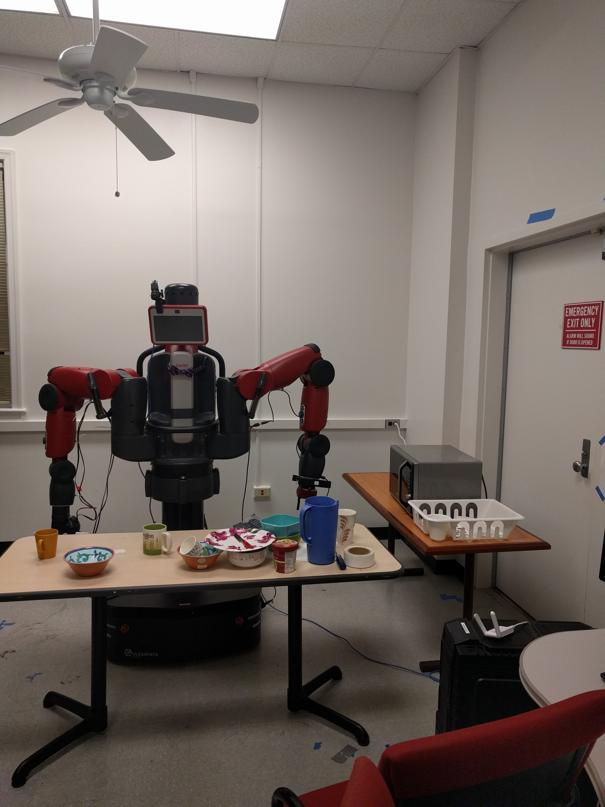
\includegraphics[width= 70mm]{images/5.jpg}
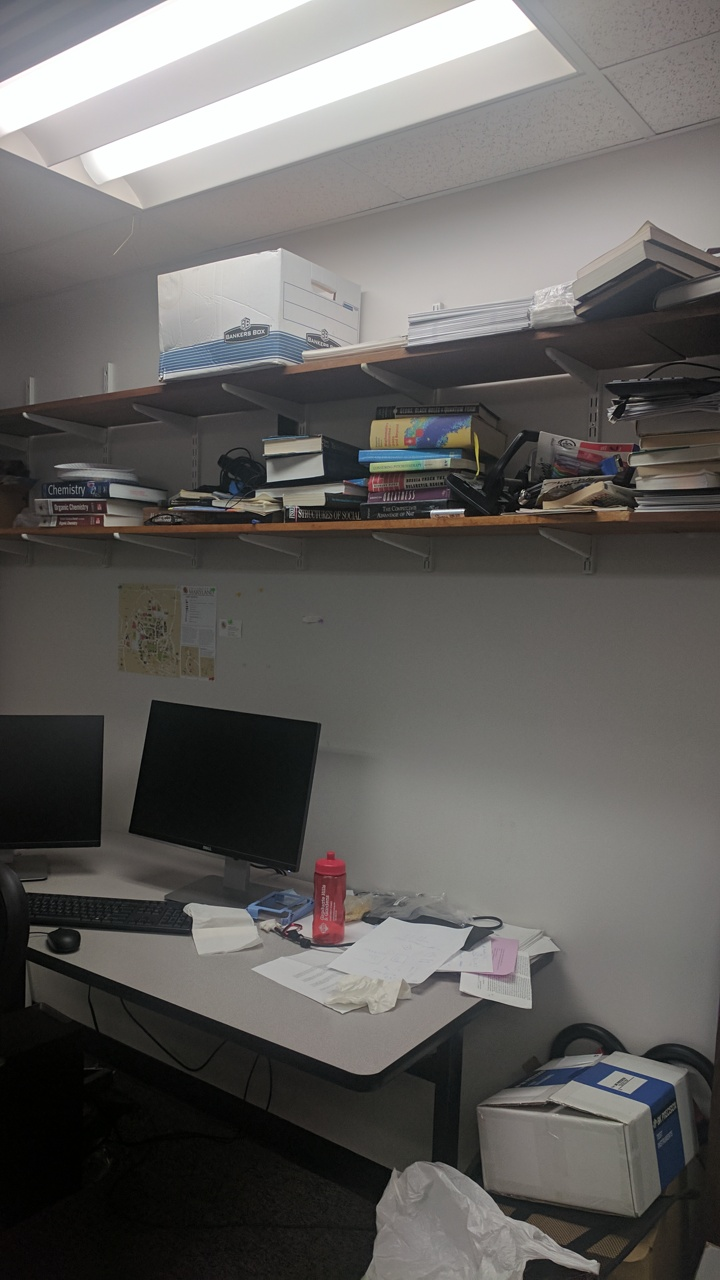
\includegraphics[width= 73mm]{images/6.jpg}
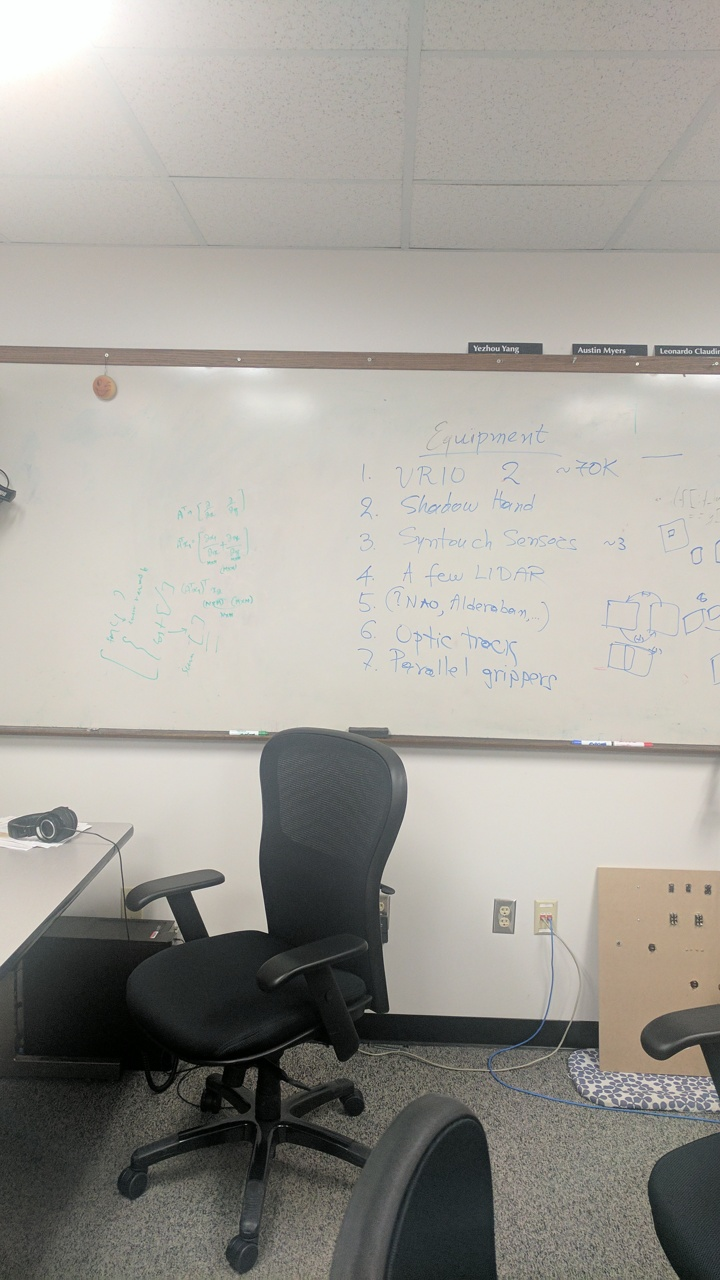
\includegraphics[width= 70mm]{images/7.jpg}
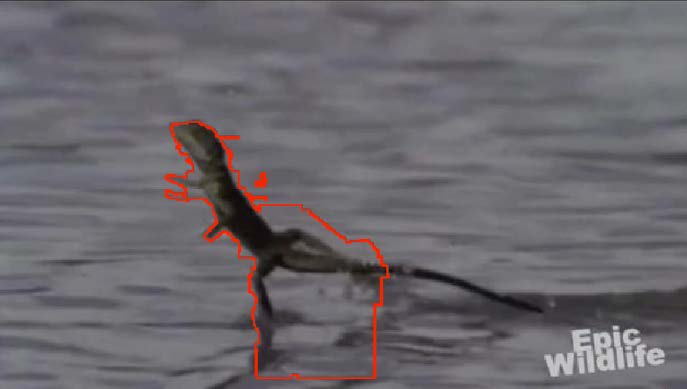
\includegraphics[width= 73mm]{images/8.jpg}
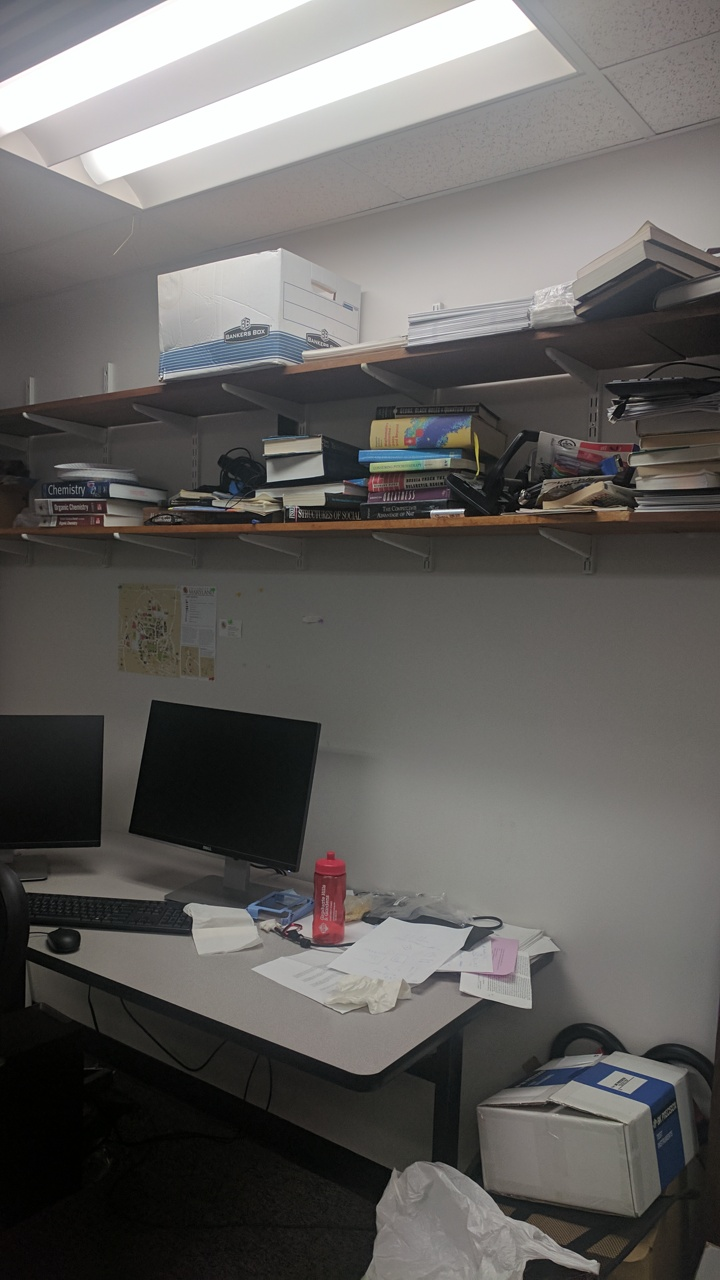
\includegraphics[width= 70mm]{images/9.jpg}
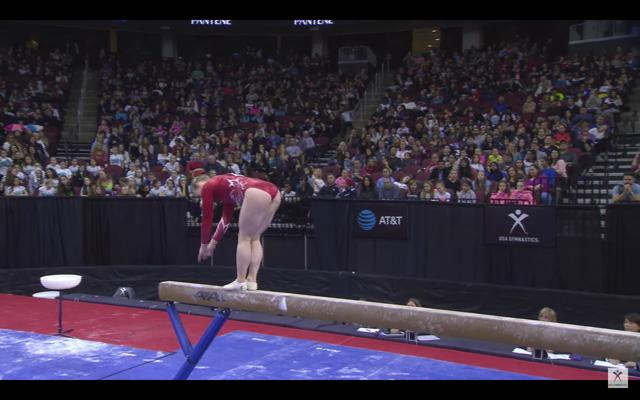
\includegraphics[width= 73mm]{images/10.jpg}






\section{Work Distribution}
\subsection{Yizhan Ao}
Setup Local Windows + Initialize Color Models + Combine Shape and Color Models + Merge Local Windows + Extract final foreground mask + Update Color Model (and color confidence)+ Report(1-6)
\subsection{Yingqiao Gou}
Compute Color Model Confidence + Initialize Shape Model + Compute Shape confidence + Estimate Entire-Object Motion + Estimate Local Boundary Deformation(6-12)

\section{Output}
We stored the videos into the folder outputs

\section{Conclusion}
This is a pretty cool project. I have to admit that the papers are very helpful to understand the concept here. 

The turtle's solid blue background allowed it to focus on its features. Because the color distribution of the backdrop is virtually always the same throughout, solid backgrounds are easy to discern from an item of focus. Furthermore, the turtle never strayed far from its initial location.

However the biker fails since the speed it left the frame. The feature windows to follow that too off from the background

The beam gymnast has a huge noise in the background. In that case we need to estimate the movement frame by frame 

The weight lifting video has moved the center of the body, and the identification only focus on part of the drum.
% \begin{figure}[H]
% \centering

% \begin{subfigure}{.5\textwidth}
%   \includegraphics[height=30mm\linewidth,right]{images/step controlled.png}
%   \caption{QNN with Step Controlled structure with 2 step-control connections [7]}
%   \label{fig:sub2}
% \end{subfigure}
% % \caption{A figure with two subfigures}
% \label{fig:test}
% \end{figure}


\section*{References}
\small
\begin{hangparas}{.25in}{1}
[1] Bai, X., Wang, J., Simons, D. and Sapiro, G., 2009, July. Video snapcut: robust video object cutout using localized classifiers. In ACM Transactions on Graphics (ToG) (Vol. 28, No. 3, p. 70). ACM.
\end{hangparas}

\begin{hangparas}{.25in}{1}
[2] Wang, J. and Cohen, M.F., 2005, October. An iterative optimization approach for unified image segmentation and matting. In Computer Vision, 2005. ICCV 2005. Tenth IEEE International Conference on (Vol. 2, pp. 936-943). IEEE.
\end{hangparas}

\end{document}
